\icode{E-MI-MU-L3-261105-002}
（多选）
一质量为\(M\)斜劈静止于粗糙的水平地面上，在其斜面上放一滑块\(m\)，若给\(m\)一向下的初速度\(v_0\)，则\(m\)正好保持匀速下滑。如图所示，现在\(m\)下滑的过程中再加一个作用力，则以下说法正确的是\paren[]

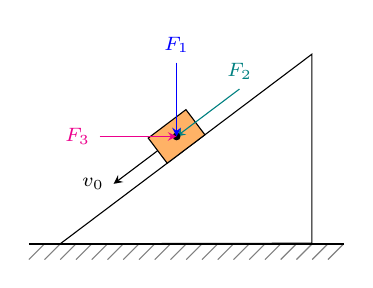
\begin{tikzpicture}[>=stealth,font=\scriptsize]
	\begin{scope}[rotate=37]
		\coordinate (O) at(2,.2);
		\draw (0,0)--(4,0)--++(-127:2.4)--(0,0);
		\draw[fill=orange!60] (1.7,0) rectangle(2.3,.4);
		\draw[->] (1.7,.2)--(1,.2)node[left]{\(v_0\)};
		\draw[->,teal] (3,.2)node[above]{\(F_2\)}--(2,.2);
	\end{scope}
	\fill (O) circle(.05);
	\draw[->,blue] (O|-1.5,2.3)node[above]{\(F_1\)}--(O);
	\draw[->,magenta] (O-|0.5,.3)node[left]{\(F_3\)}--(O);
	\foreach \x in {-.4,-.2,...,3.4}
		\draw[gray] (\x,-.2)--++(.2,.2);
	\draw[thick] (-.4,0)--(3.6,0);
\end{tikzpicture}
\begin{choices}
	\item 在\(m\)上加一竖直向下的力\(F_1\)，则\(m\)将保持匀速运动，\(M\)对地无摩擦力的作用
	\item 在\(m\)上加一个沿斜面向下的力\(F_2\)，则\(m\)将做加速运动，\(M\)对地有水平向左的静摩擦力的作用
	\item 在\(m\)上加一个水平向右的力\(F_3\)，则\(m\)将做减速运动，在\(m\)停止前\(M\)对地有向右的静摩擦力的作用
	\item 无论在\(m\)上加什么方向的力，在\(m\)停止前\(M\)对地都无静摩擦力的作用
\end{choices}
\begin{answer}
	AD\qquad 提示：
\end{answer}